	\documentclass[../pfc.tex]{subfiles}
	
	\begin{document}
	
	
	\section{Parte App móvil}
	
	\section{Arquitectura}
	
	Como se ha comentado antes en este documento Scrum y las tecnologías ágiles, por su forma de enfocar las tareas y el propio desarrollo, si no se introducen medidas paliativas que corrijan esto, suelen obtener diseños arquitecturales de clases un poco pobres, tendentes al acoplamiento y poco cohesionado. Para paliar esto se suelen introducir historias de usuario de reducción de deuda técnica, o de refactorización de todo el código existente, así como herramientas que detecten "code smells"(cita o algo) o malas practicas de desarrollo. Estas herramientas de análisis estático de código pueden advertirnos sobre puntuales problemas dentro de una clase, pero poco hay a nivel de las relaciones entre las mismas, fuera del uso de patrones de diseño conocidos, y aun en las relaciones entre estos patrones que son bloques más grandes de código. Es por eso que creemos que hay que establecer unas líneas base al principio del proyecto sobre la arquitectura de la propia aplicación. En principio serán ciertamente vaguedades y lugares comunes sobre el desarrollo en capas, aislamiento de las mismas etc, pero si a través de los sprints reservamos un poco de tiempo en la reunión de sprint planning para conversar sobre las historias del propio sprint, en que capa encajan, como deberían hablar las capas entre sí si son mas de una las involucradas en la historia, etc ademas de con las historias de deuda técnica si fuesen necesarias creemos que puede solventarse en gran medida esa falta de bueno diseño y arquitectura que se achaca a las metodologías ágiles.\\
	
	Para hablar de arquitectura hemos tomado como referencia Clean Architecture(cita) propuesta por Robert C. Martin aunque es muy similar a la Arquitectura Cebolla de Kent Beck (comprobar) o la Arquitectura Hexagonal de Alaister Cockburn. Todas ellas se basan por hacer capas fuertemente cohesionadas dentro de cada una pero con nulo conocimiento fuera de las mismas que se comunican mediante interfaces públicos ofrecidos al resto de capas. Esto y la propagación hacia el interior, esto es que cada capa solo hablara con la que tiene arquitecturalmente en un nivel superior o inferior. Esto es la capa de UI que es la que interactuá con el usuario solamente invocará métodos de la interfaz de la capa de vista que es la que conceptualmente tiene justo encima. Esta solamente interactuará con la capa de UI antes mencionada y con la capa del presentador, y así sucesivamente. 
	
	
	
	\section{Tecnología}
	
	\section{Diagrama de Clases}
	
	\section{Diseño de la base de datos}
	
	\section{Diagramas de estado}
	
	\section{Prototipado}
	
	En la fase de diseño, el propósito del prototipo es obtener una primera versión de la apariencia de la interfaz de usuario así como de la funcionalidad incluida (mostrar las ventanas, su navegación, interacción, controles y botones). Con esto se pretende que el cliente tenga una primera toma de contacto con la futura aplicación antes de su desarrollo final, para así reducir o eliminar todas aquellas disconformidades y cambios en fases futuras.
	
		\subsection{Material Design}
		Material Design es la nueva metáfora visual de Matias Duarte para el sistema operativo móvil Android, en su version 5.0 y posteriores, y todo el ecosistema Google en web y supone una pequeña ruptura con la anterior metáfora de Android llamada Holo. 
		
		Es un diseño donde la profundidad, las superficies, los bordes, las sombras y los colores juegan un papel principal.
		
		Precisamente este diseño basado en objetos es una manera de intentar aproximarse a la realidad, algo que en un mundo donde todo es táctil y virtual es difícil. Material Design quiere guiarse por las leyes de la física, donde las animaciones sean lógicas, los objetos se superpongan pero no puedan atravesarse el uno al otro y demás.
		
		Material Design es un diseño con una tipografía clara, casillas bien ordenadas, colores e imágenes llamativos para no perder el foco y un sentido del orden y la jerarquía muy marcado. Estas ideas ya se aplican en muchos diseños, pero en Material Design Google ha creado unas normas muy claras de como llevarlo a la práctica.
		
		\subsection{Pantallas Principales}
		
			Pantallas iniciales y flujo de la aplicación que de manera inicial hemos planteado para la misma.
			No es la versión final de la aplicación pero si se aproxima y nos da una idea clara de lo que debería ser o a lo que debería parecerse.
			Estos prototipos, sirven para orientarnos a la hora de construir la aplicación
			
			\textbf{Pantalla Principal y Drawer menú}
			El usuario, al ejecutar la aplicación accede a una pantalla cuyo contenido es el listado de las actividades próximas a realizar, ya sea una cita médica o una rutina.
			El drawer nos permite navegar entre actividades, desde la pantalla principal podemos añadir citas y acceder de manera individual a las mismas.
			 
			
			\begin{figure}
				\centering
				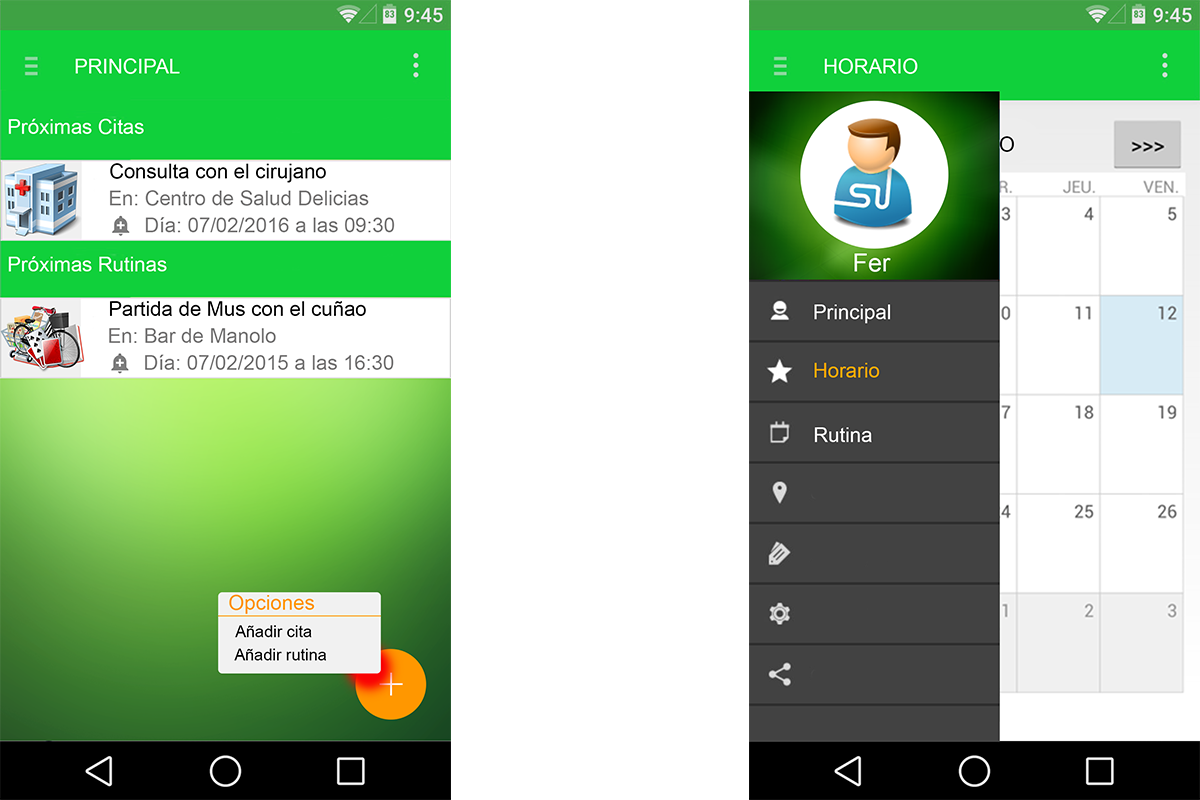
\includegraphics[width=0.7\linewidth]{../images/principal_2}
				\caption[Drawer menú y Pantalla principal]{Descripción de la pantalla principal y Drawer menú}
				\label{fig:principal}
			\end{figure}
			
			
			\textbf{Pantallas referentes a la programación de actividades}
			Desde estás pantallas tenemos una visión de la ocupación diaria del paciente y de la ocupación mensual, desde la vista mensual al menos se podrán añadir nuevas citas médicas o rutinas para ese paciente.

			
			\begin{figure}
				\centering
				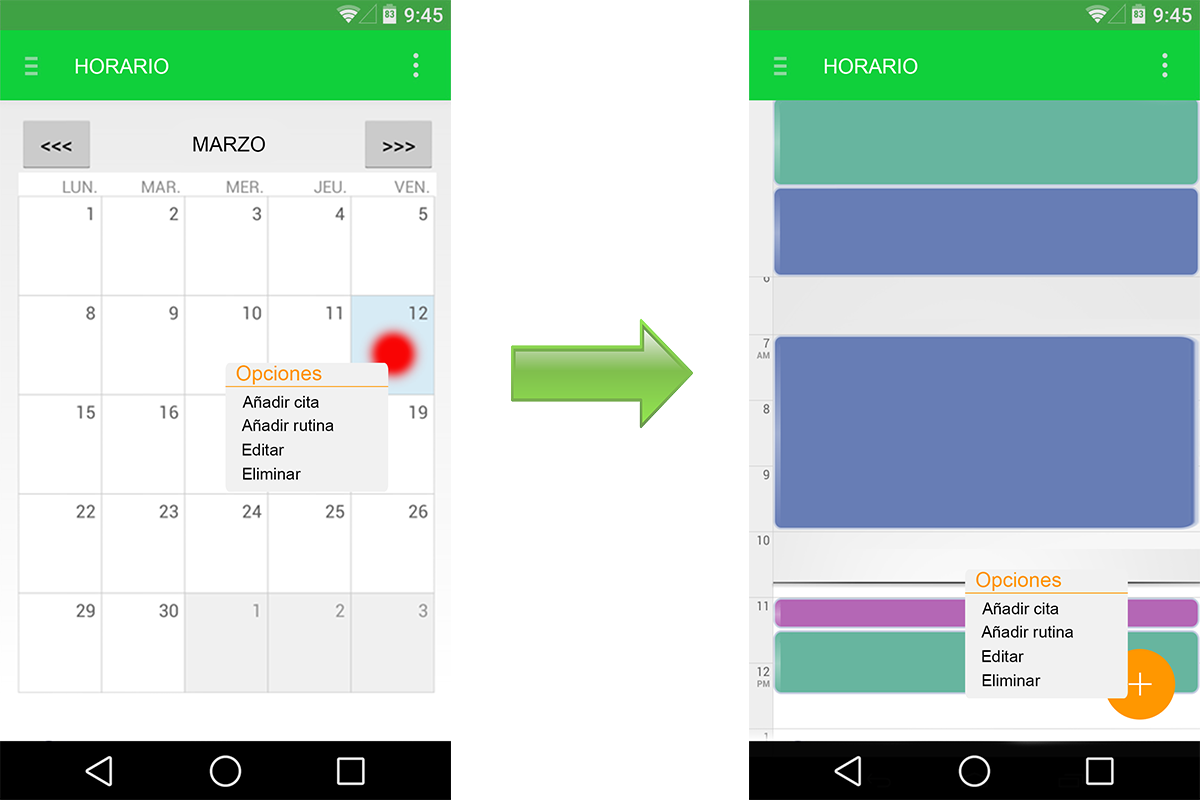
\includegraphics[width=0.7\linewidth]{../images/horario_2}
				\caption{Pantallas con los horarios y ocupación del paciente}
				\label{fig:horario_2}
			\end{figure}
			
			
			\textbf{Pantallas referentes a la rutina diaria}
			Listado de las rutinas diarias que tiene ese paciente y representación de la introducción de una nueva rutina para ese paciente.
			Dentro de la introducción de la rutina se podrán añadir nuevos personajes que acompañarán a ese paciente y le harán más fácil recordar con quien quedó y para qué.

			
			\begin{figure}
				\centering
				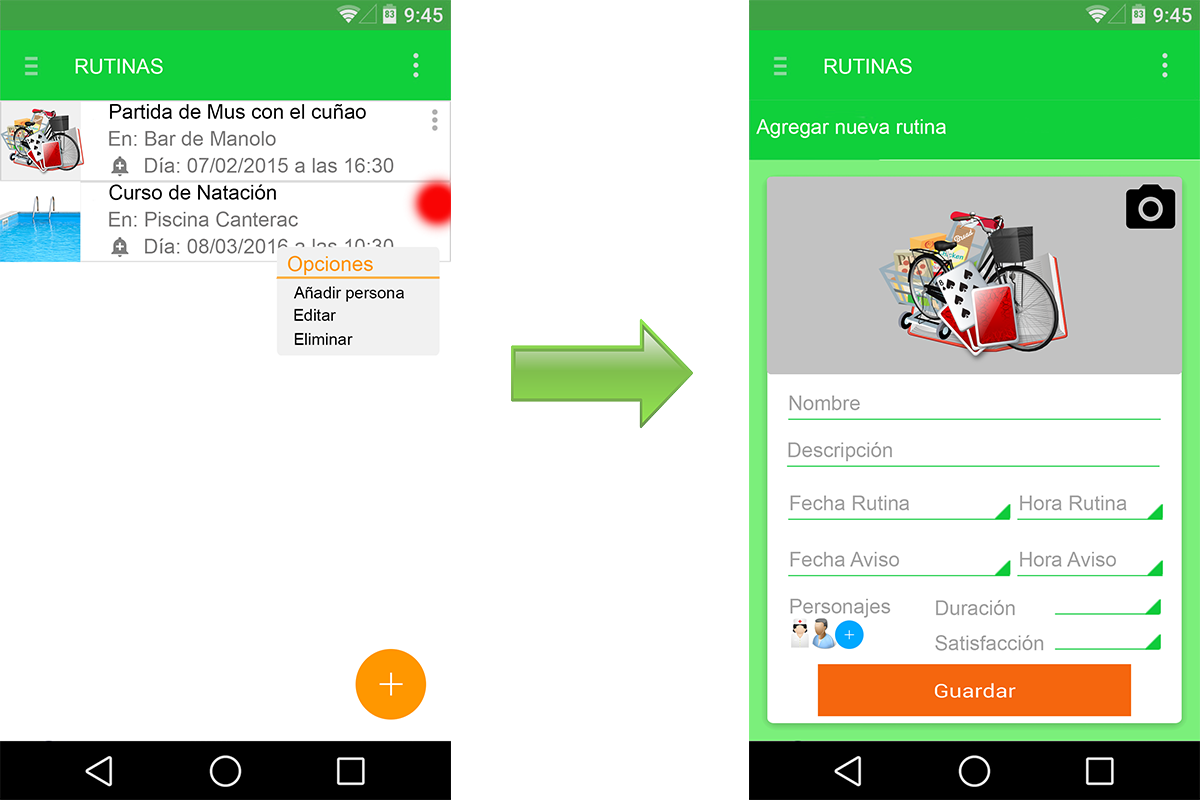
\includegraphics[width=0.7\linewidth]{../images/rutina}
				\caption{Pantalla con la interfaz para las rutinas}
				\label{fig:rutina}
			\end{figure}
						
			
			\textbf{Pantallas referentes a las citas médicas}
			Listado de las citas medicas de ese paciente e introducción de la cita en si de manera individual.
			De funcionamiento similar a las pantallas anteriores pero con diferencias sustanciales en la funcionalidad de la introducción de información, se pueden añadir personajes, síntomas, medicamentos y pruebas, de manera que el paciente cuando acuda a la cita lleve de manera ordenada toda esta información.
			
			\begin{figure}
				\centering
				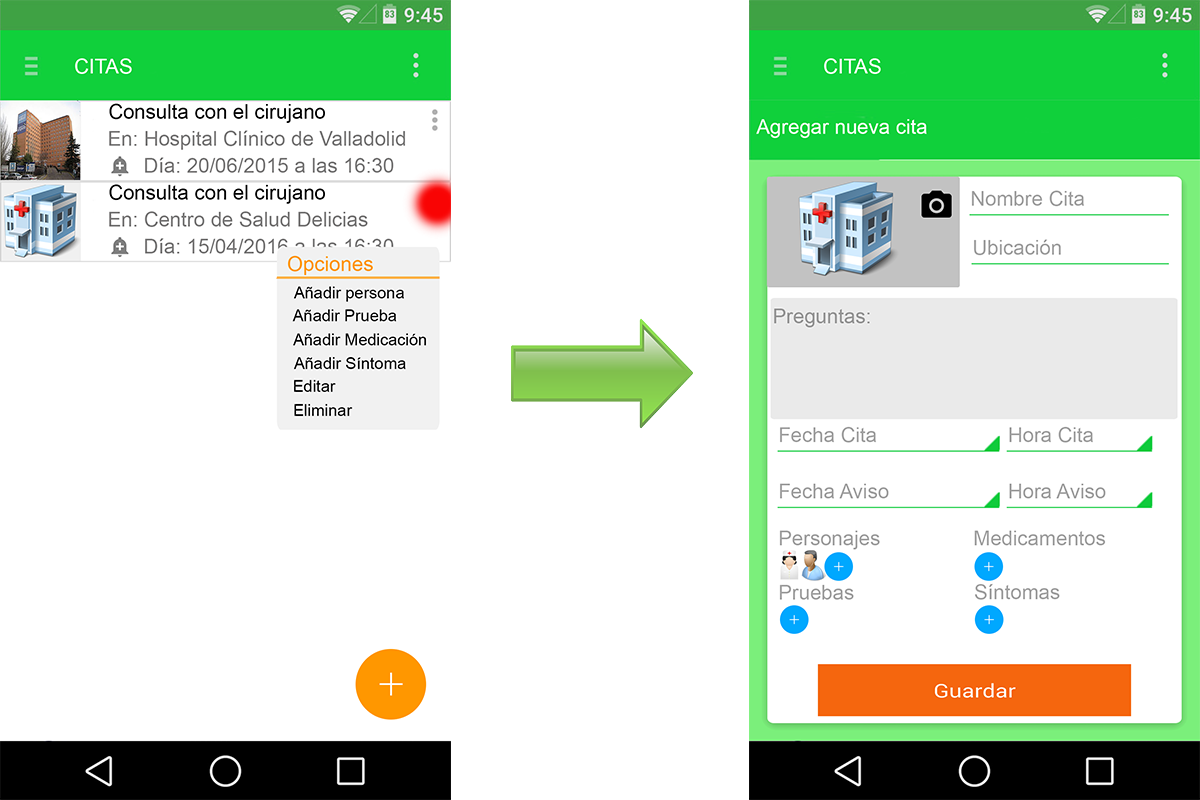
\includegraphics[width=0.7\linewidth]{../images/citas}
				\caption{Pantalla con la actividad de las citas}
				\label{fig:citas}
			\end{figure}
			
			
			\textbf{Pantallas referentes a la medicación}
			El usuario introduce los medicamentos que toma, de manera que puede añadir alertas a los mismos para que se le avise de que ha llegad la hora de la dosis con una notificación.
			Se podrán introducir otros datos del medicamento como pueden ser los intervalos entre dosis, indicaciones...
			
			\begin{figure}
				\centering
				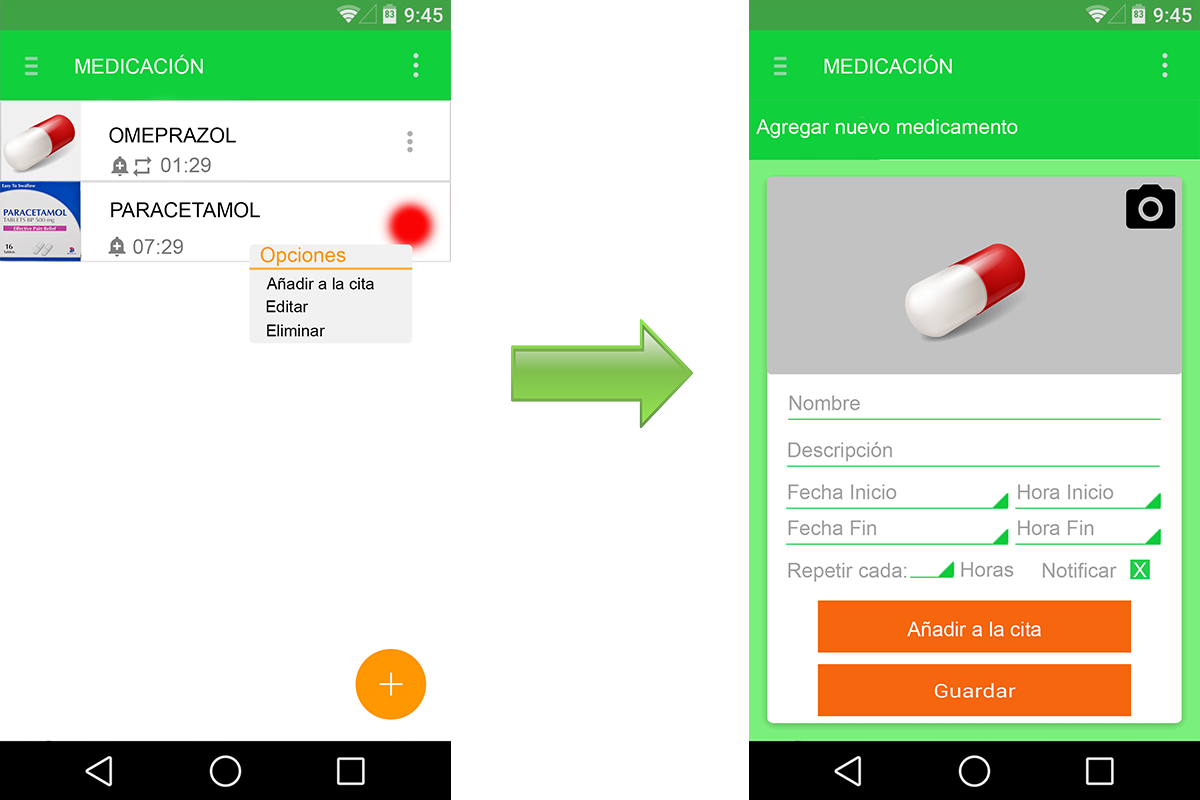
\includegraphics[width=0.7\linewidth]{../images/medicacion}
				\caption{Pantalla con la actividad de la medicación}
				\label{fig:medicacion}
			\end{figure}
			
			
			\textbf{Pantallas de gestión de personajes}
			El usuario puede añadir a la aplicación su lista de amigos, personal médico que le atiende, asistentes, etc, con sus datos personales, de manera que a la hora de hacer una rutina (actividad) o acudir a una cita, puedan ser añadidos.
			
			
			\begin{figure}
				\centering
				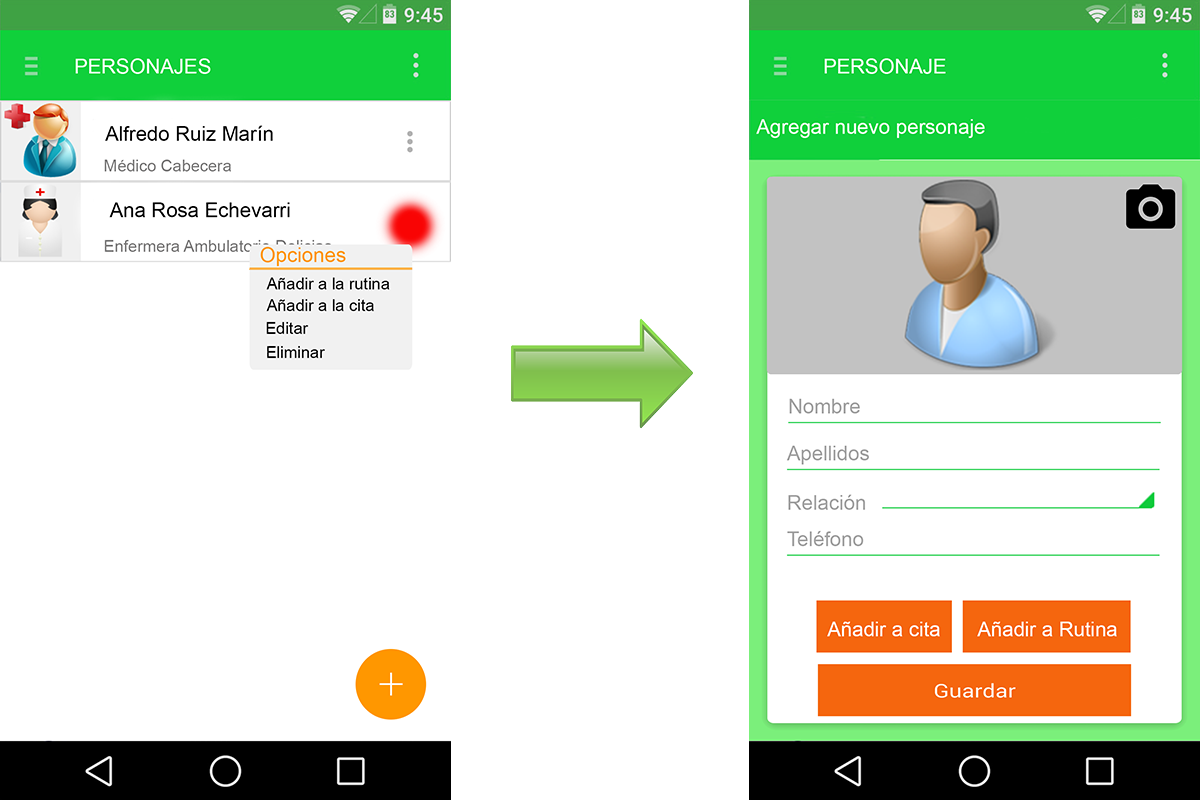
\includegraphics[width=0.7\linewidth]{../images/personajes}
				\caption{Pantalla con la actividad de los personajes}
				\label{fig:personajes}
			\end{figure}
			
			
			\textbf{Pantallas de gestión de pruebas médicas}
			Se facilita el poder llevar las pruebas médicas en forma de archivo fotográfico para poder consultarse en alguna de las citas medicas a las que acuda, tales como revisiones, visitas al fisio, a la enfermera. Listado del mismo.
			
			\begin{figure}
				\centering
				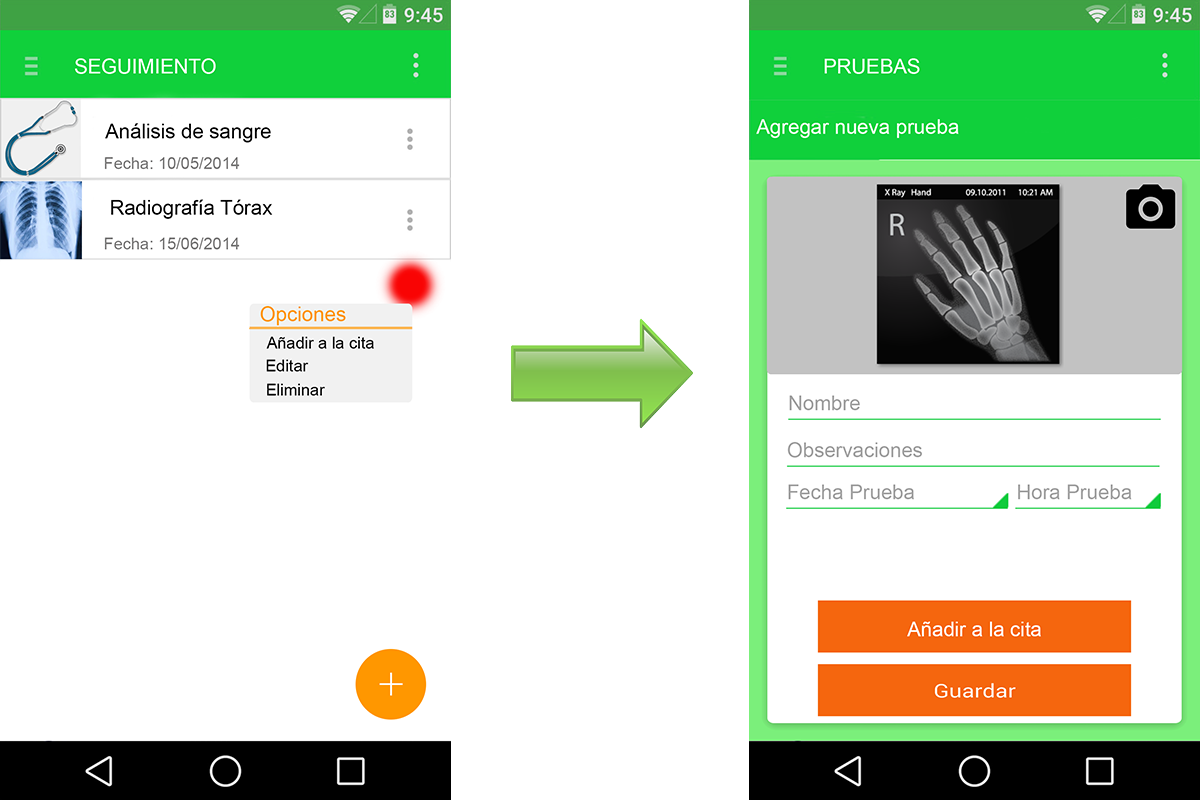
\includegraphics[width=0.7\linewidth]{../images/pruebas}
				\caption{Pantalla con la actividad de las pruebas}
				\label{fig:pruebas}
			\end{figure}
			
			
			\textbf{Pantallas de gestión de los síntomas}
			El usuario puede tomar nota de los síntomas, molestias, efectos secundarios negativos o positivos que le acontecen, para poder asignarles después a una cita médica y poder completar de manera más eficiente las mismas, pudiendo aportar información adicional que ayude a su médico a mejorar el diagnóstico.
			
			\begin{figure}
				\centering
				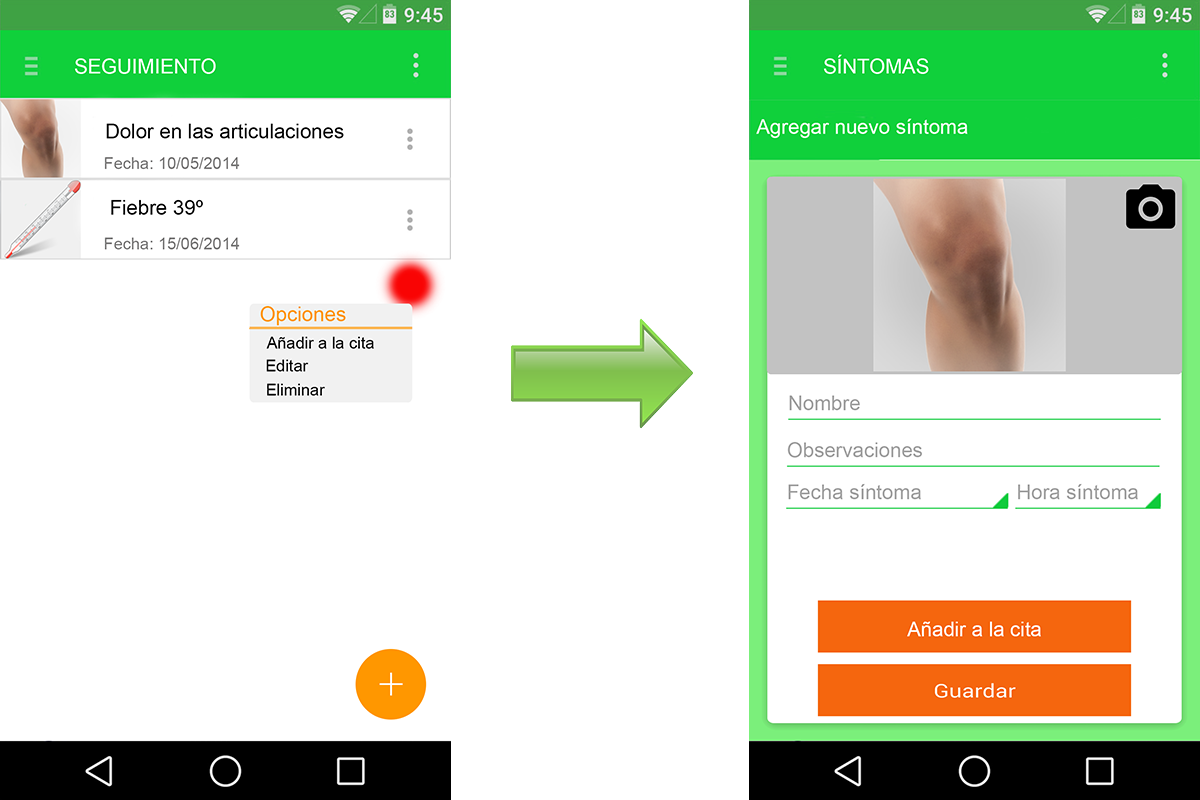
\includegraphics[width=0.7\linewidth]{../images/sintomas}
				\caption{Pantalla con la actividad de los síntomas}
				\label{fig:sintomas}
			\end{figure}
			
			
			\textbf{Pantallas de Recursos}
			Estas pantallas están pensadas para que el paciente disponga de ayuda adicional, y una serie de recursos de fácil acceso así como una sección de noticias de la AECC para que puedan ser consultadas por el paciente.
			Sección de meditación, consejos generales que le puedan ser de ayuda, noticias y teléfonos de interés. 
			
			\begin{figure}
				\centering
				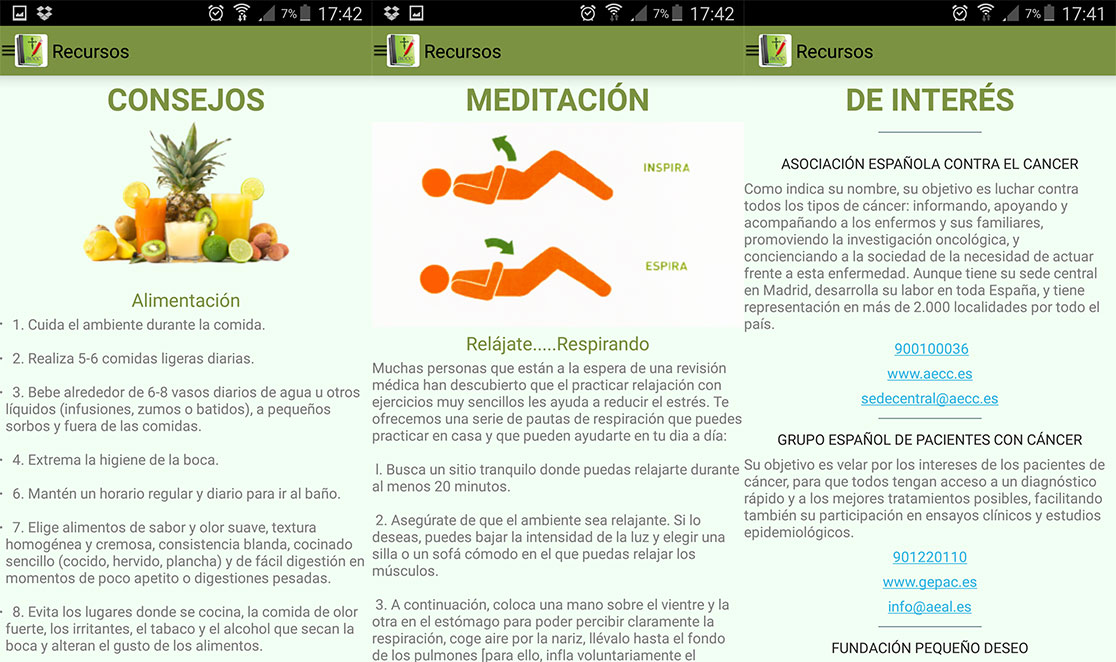
\includegraphics[width=0.7\linewidth]{../images/recursos}
				\caption{Pantalla con la actividad de los recursos}
				\label{fig:recursos}
			\end{figure}
			
			
			\textbf{Pantalla de perfil de usuario}
			El usuario podrá introducir sus datos personales para que la aplicación pueda tratarle de manera personalizada.
			
			\begin{figure}
				\centering
				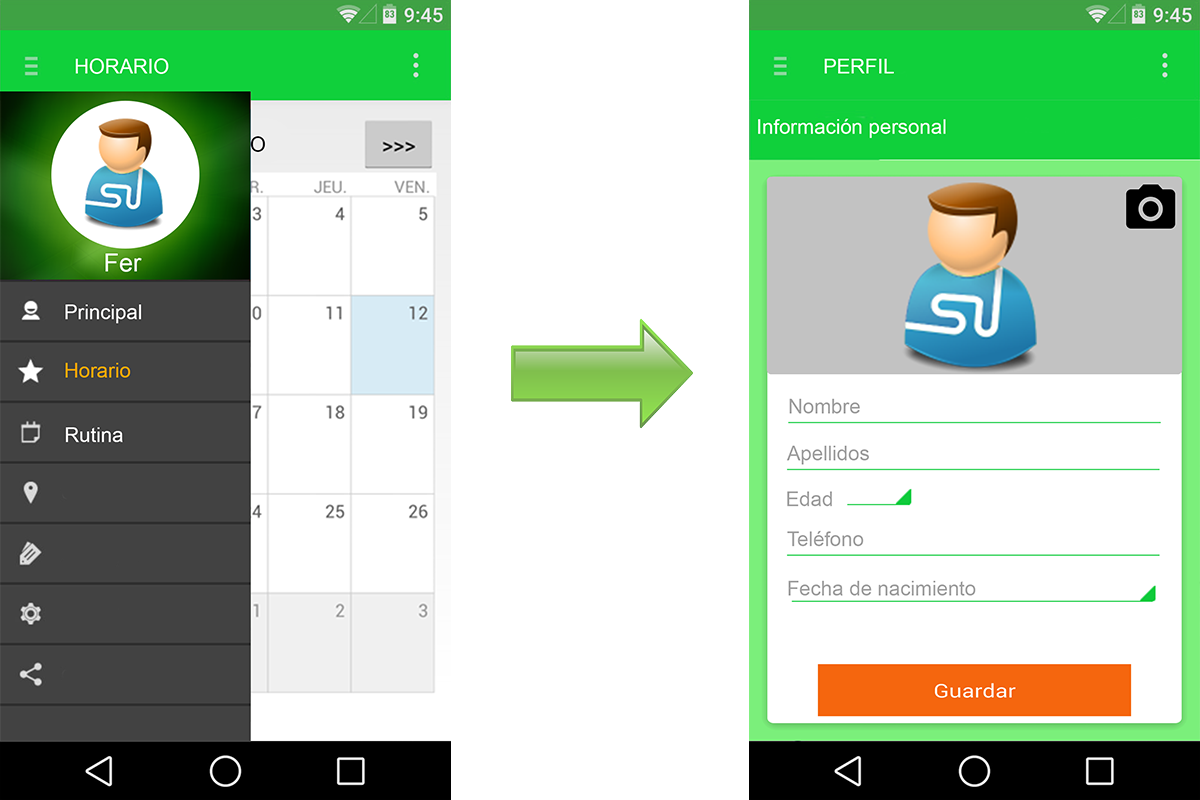
\includegraphics[width=0.7\linewidth]{../images/perfil_2}
				\caption{Pantalla con la actividad conf del perfil}
				\label{fig:perfil_2}
			\end{figure}
			
			
			\textbf{Otros: Pantalla de presentación y carga}
			Pantalla inicial de carga, se utiliza para aportar más identidad a la aplicación y a modo de pequeña intro.
			
			\begin{figure}
				\centering
				
\includegraphics[width=0.3\linewidth]{../images/flasher_pantalla_carga}
				\caption{Pantalla con la actividad de las citas}
				\label{fig:flasher_pantalla_carga}
			\end{figure}
			
			
		
	\section{Flujo de navegación}
	
	
\end{document}